\section{Results}
\label{sec:results}

\subsection{Source-Level Divergence}
\label{sec:source_results}

\begin{table}[t]
\centering
\caption{Source-level forward KL summaries. KL is $\klinstbase$ over teacher-forced next-token distributions. The largest value in each numeric column is bolded.}
\label{tab:source_stats}
\resizebox{\textwidth}{!}{%
\begin{tabular}{@{}lrrrrr@{}}
\toprule
\textbf{Source} & \textbf{Mean KL} & \textbf{Median KL} & \textbf{P90 KL} & \textbf{P99 KL} & \textbf{Top-1 disagree} \\
\midrule
\justeval & \textbf{0.109} & \textbf{0.063} & \textbf{0.271} & 0.585 & \textbf{0.187} \\
\beavertails & 0.104 & 0.043 & 0.208 & 1.237 & 0.150 \\
\wikitext & 0.096 & 0.042 & 0.184 & 1.145 & 0.131 \\
\arena & 0.084 & 0.035 & 0.176 & \textbf{1.260} & 0.131 \\
\alpaca & 0.071 & 0.031 & 0.172 & 0.559 & 0.128 \\
\bottomrule
\end{tabular}
}
\end{table}


\begin{figure}[t]
\centering
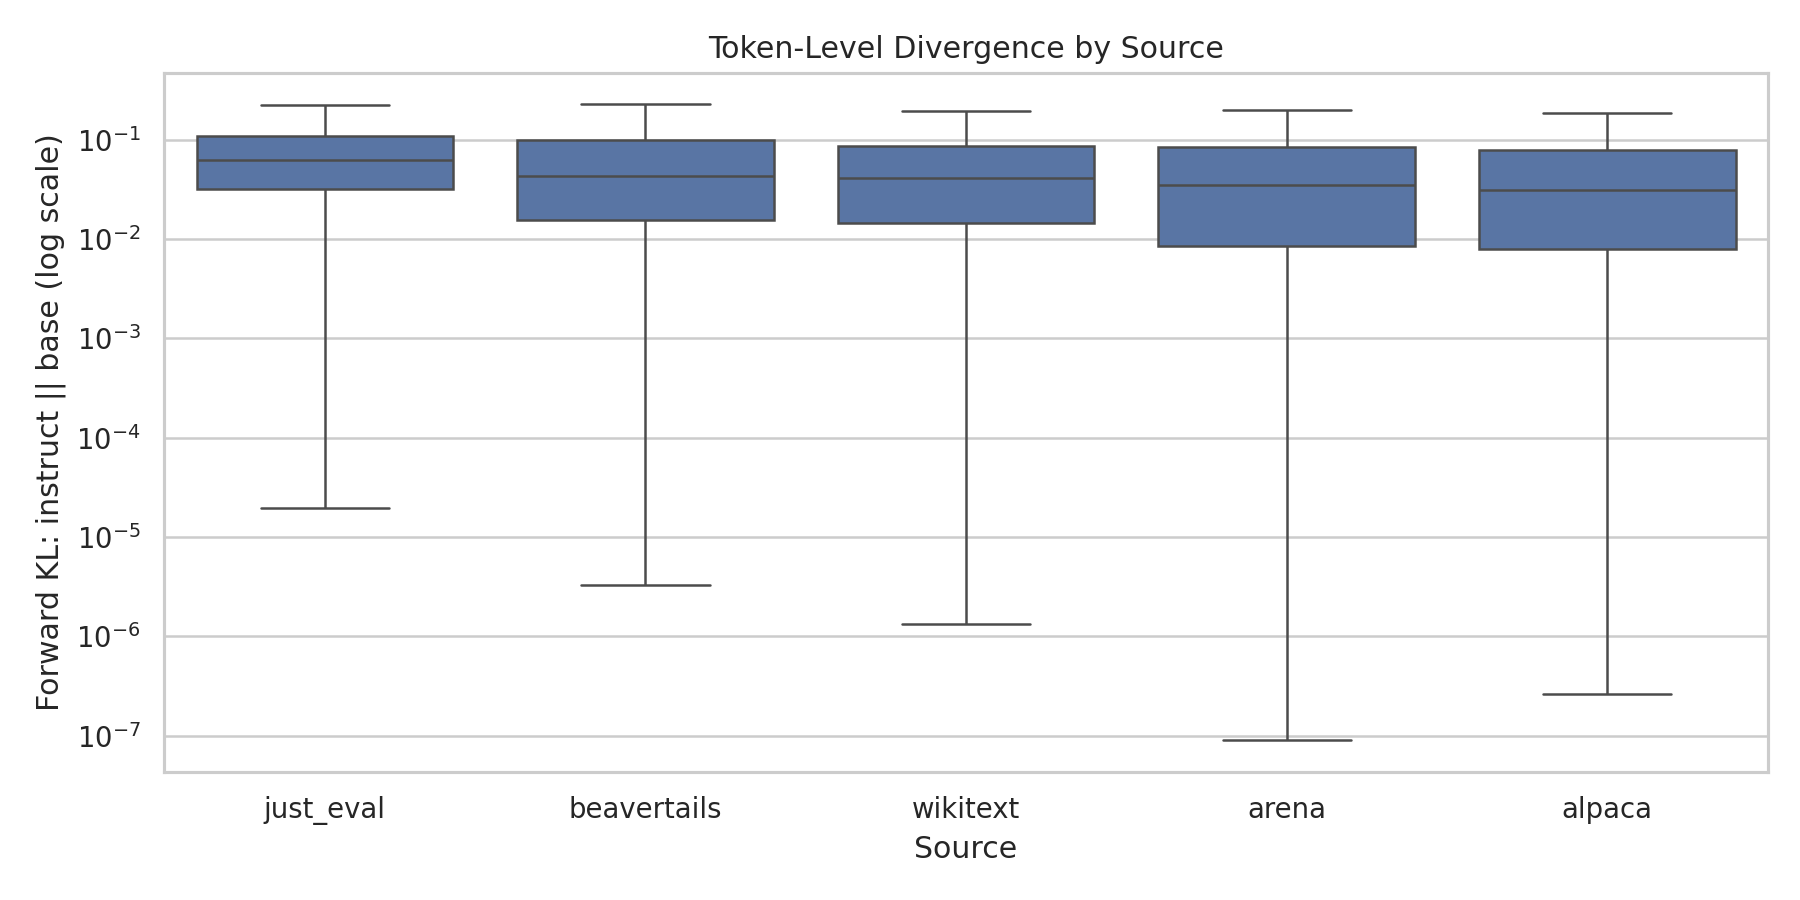
\includegraphics[width=0.48\linewidth]{figures/kl_by_source.png}
\hfill
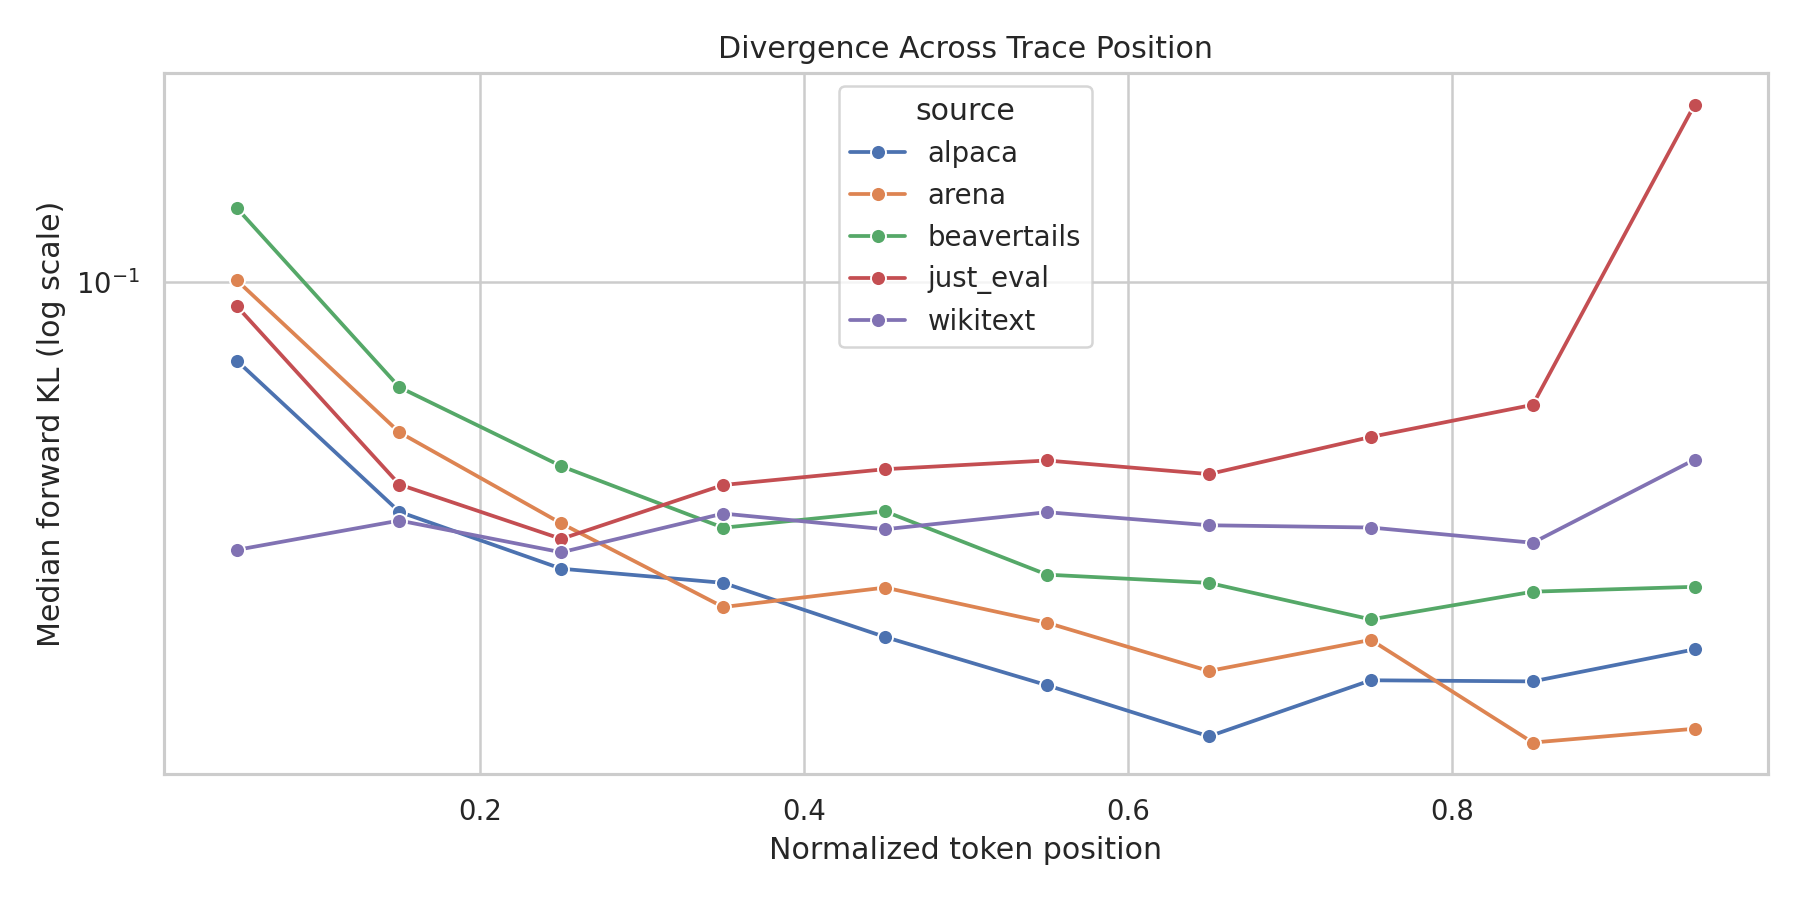
\includegraphics[width=0.48\linewidth]{figures/kl_position_trend.png}
\caption{Token-level KL by source and position. \figleft shows that \justeval has the largest mean KL and top-1 disagreement, while \alpaca has the lowest mean KL. \figright shows that divergence is concentrated near boundaries and early positions rather than being uniform across traces.}
\label{fig:kl_landscape}
\end{figure}

\tabref{tab:source_stats} reports divergence by source. Mean forward KL ranges from 0.071 for \alpaca to 0.109 for \justeval. The top-1 disagreement rate follows a similar pattern: \justeval has the largest disagreement rate at 0.187, while \alpaca has the lowest at 0.128. These values confirm that instruction and boundary-heavy sources are more divergent on average, but the differences are not limited to prompt datasets. \wikitext, a natural-text baseline, has mean KL 0.096 and a P99 KL of 1.145.

Generation-start positions are much more divergent than ordinary continuations. As shown in \tabref{tab:generation_start}, \beavertails has generation-start mean KL 0.802 and P90 KL 2.085, compared with a source-wide mean KL of 0.104. \arena, \alpaca, and \justeval also show elevated generation-start KL. This supports the view that response boundaries are a major site of instruction-tuning shift.

\begin{table}[t]
\centering
\caption{Generation-start divergence by source. Boundary positions are substantially more divergent than average continuations, especially for \beavertails. The largest value in each metric is bolded.}
\label{tab:generation_start}
\begin{tabular}{@{}lrrr@{}}
\toprule
\textbf{Source} & \textbf{Mean KL} & \textbf{Median KL} & \textbf{P90 KL} \\
\midrule
\beavertails & \textbf{0.802} & \textbf{0.504} & \textbf{2.085} \\
\arena & 0.444 & 0.414 & 0.846 \\
\alpaca & 0.355 & 0.296 & 0.627 \\
\justeval & 0.352 & 0.272 & 0.688 \\
\wikitext & 0.159 & 0.095 & 0.262 \\
\bottomrule
\end{tabular}
\end{table}


\begin{table}[t]
\centering
\caption{Strongest source-level Mann-Whitney comparisons on per-example mean KL after Holm correction. Cliff's delta is for the first source relative to the second.}
\label{tab:source_tests}
\begin{tabular}{@{}lrrrr@{}}
\toprule
\textbf{Comparison} & \textbf{Mean A} & \textbf{Mean B} & \textbf{Holm $p$} & \textbf{Cliff's $\delta$} \\
\midrule
\alpaca vs. \justeval & 0.0898 & 0.1131 & \textbf{0.000087} & -0.471 \\
\alpaca vs. \beavertails & 0.0898 & 0.1230 & 0.00710 & -0.356 \\
\bottomrule
\end{tabular}
\end{table}


At the per-example level, the strongest Holm-corrected source differences are \alpaca versus \justeval and \alpaca versus \beavertails. The \alpaca-vs-\justeval comparison has Holm-corrected $p=8.66 \times 10^{-5}$ and Cliff's delta $-0.471$; the \alpaca-vs-\beavertails comparison has Holm-corrected $p=0.00710$ and Cliff's delta $-0.356$. Most other pairwise source differences do not remain significant after correction, including \arena versus \wikitext.

\subsection{Predicting Token-Level KL}
\label{sec:predictor_results}

\begin{table}[t]
\centering
\caption{Held-out predictor performance on $\log(1+\klinstbase)$. Lower is better for MAE and RMSE; higher is better for $R^2$ and Spearman correlation. Best values are bolded.}
\label{tab:predictor_results}
\begin{tabular}{@{}lrrrr@{}}
\toprule
\textbf{Model} & \textbf{MAE} & \textbf{RMSE} & \textbf{$R^2$} & \textbf{Spearman $r$} \\
\midrule
\meanbaseline baseline & 0.0756 & 0.1471 & -0.0007 & n/a \\
\possource baseline & 0.0601 & 0.1256 & 0.2710 & 0.414 \\
\richpredictor & \textbf{0.0460} & \textbf{0.1183} & \textbf{0.3533} & \textbf{0.795} \\
\bottomrule
\end{tabular}
\end{table}


\begin{figure}[t]
\centering
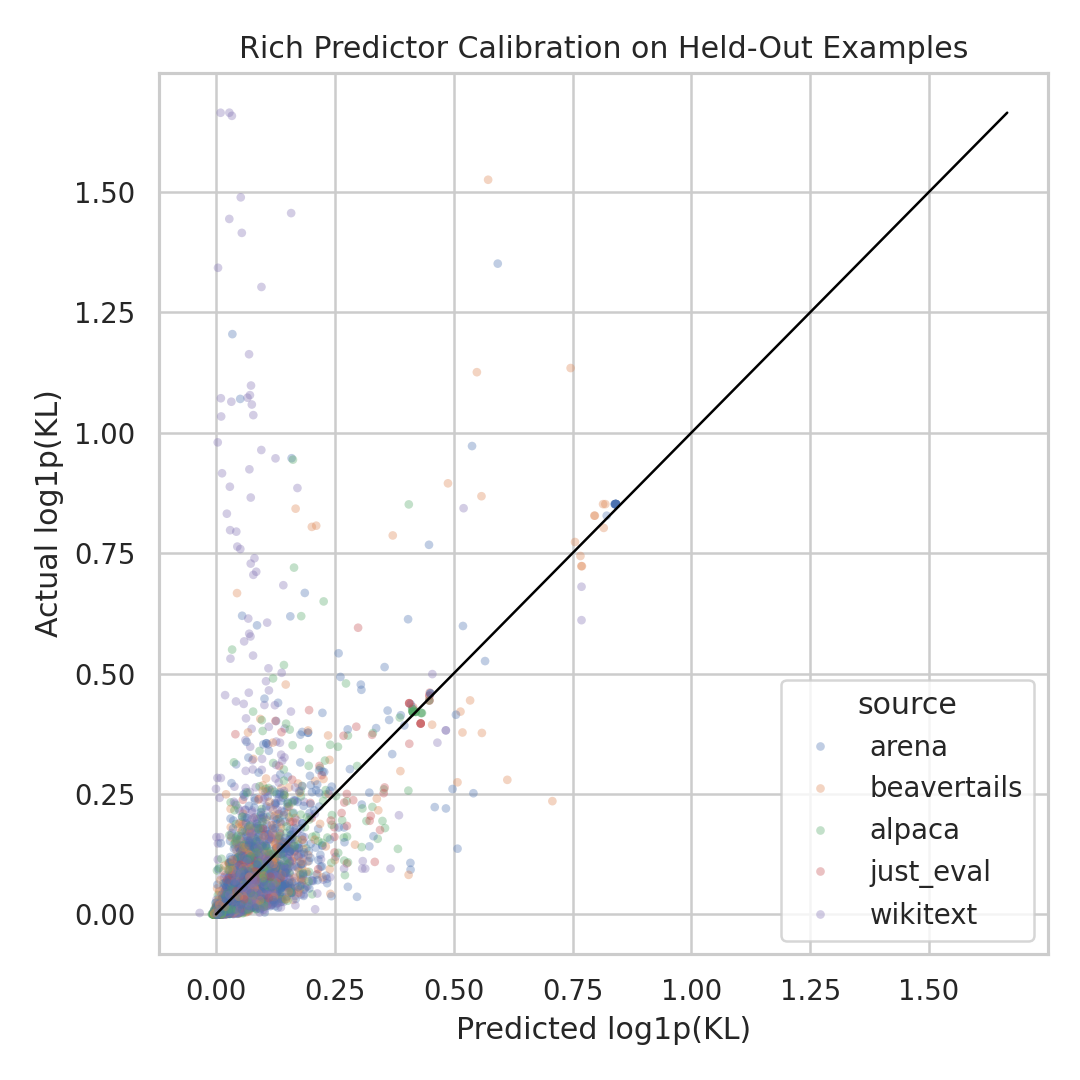
\includegraphics[width=0.48\linewidth]{figures/predictor_scatter.png}
\hfill
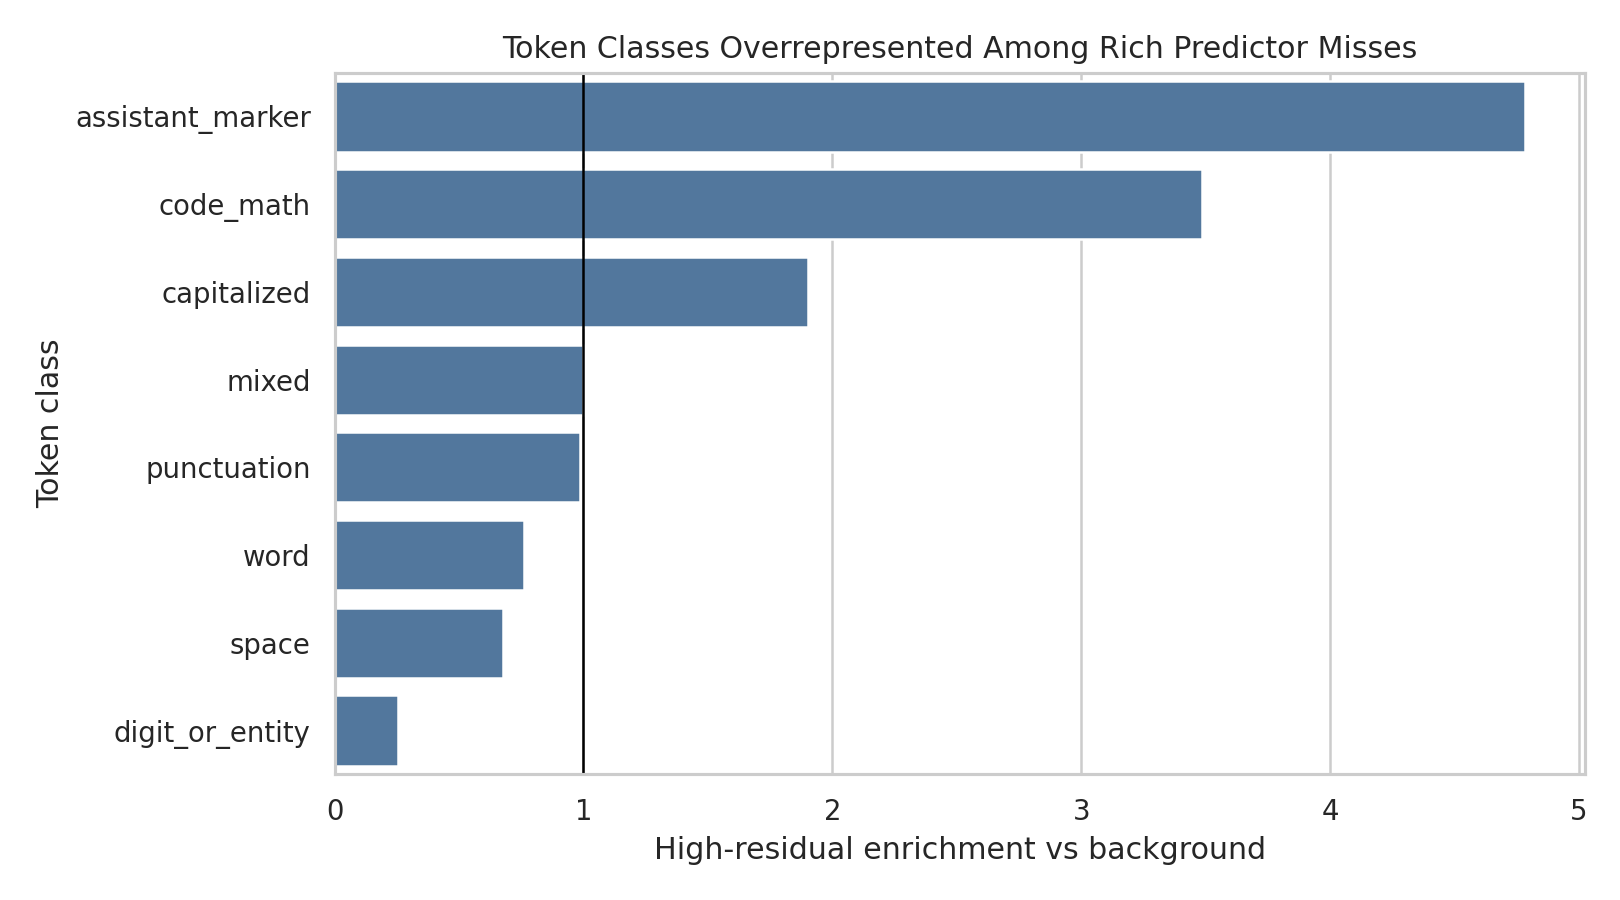
\includegraphics[width=0.48\linewidth]{figures/residual_token_class_enrichment.png}
\caption{Prediction and residual analysis. \figleft shows held-out rich-predictor predictions against actual $\log(1+\klinstbase)$. \figright shows enrichment among the top 2\% absolute residuals; known boundary and assistant-style classes are enriched, but \wikitext is also strongly overrepresented.}
\label{fig:prediction_residuals}
\end{figure}

\tabref{tab:predictor_results} shows that token-level KL is predictable above simple baselines. The \possource baseline improves MAE from 0.0756 to 0.0601 and explains 27.10\% of held-out variance. The \richpredictor further reduces MAE to 0.0460, improves RMSE to 0.1183, and raises Spearman correlation to 0.795. The grouped bootstrap mean rich-minus-position MAE difference is $-0.0142$, with a 95\% confidence interval of $[-0.0163,-0.0118]$. Because the interval is entirely below zero, the improvement is stable across held-out-example resampling.

\subsection{Residuals Identify Expected and Unexpected Shifts}
\label{sec:residual_results}

\begin{table}[t]
\centering
\caption{Enrichment among high-residual tokens. High residuals are the top 2\% of held-out tokens by absolute rich-predictor residual.}
\label{tab:residual_enrichment}
\begin{tabular}{@{}llr@{}}
\toprule
\textbf{Feature} & \textbf{Value} & \textbf{Enrichment} \\
\midrule
Segment & generation start & \textbf{5.17$\times$} \\
Token class & assistant marker & 4.78$\times$ \\
Token class & refusal style & 4.54$\times$ \\
Token class & code/math & 3.49$\times$ \\
Source & \wikitext & 3.13$\times$ \\
Token class & capitalized & 1.90$\times$ \\
\bottomrule
\end{tabular}
\end{table}


The rich predictor's median absolute residual is 0.0202. We define high-residual tokens as the top 2\% by absolute residual, corresponding to a threshold of 0.2961. \tabref{tab:residual_enrichment} shows that high residuals recover expected categories: generation starts are enriched 5.17$\times$, assistant markers 4.78$\times$, refusal-style tokens 4.54$\times$, and code/math tokens 3.49$\times$. The surprising enrichment is source-level: \wikitext tokens are enriched 3.13$\times$ among high residuals.

\begin{table}[t]
\centering
\caption{Representative rich-predictor residual failures. Residuals are actual minus predicted $\log(1+\klinstbase)$. Positive residuals indicate underprediction; negative residuals indicate overprediction.}
\label{tab:residual_examples}
\resizebox{\textwidth}{!}{%
\begin{tabular}{@{}llrrrrllp{4.2cm}@{}}
\toprule
\textbf{Source} & \textbf{Token} & \textbf{KL} & \textbf{Pred.} & \textbf{Residual} & \textbf{Agree} & \textbf{Base top-1} & \textbf{Inst. top-1} & \textbf{Interpretation} \\
\midrule
\wikitext & \texttt{is} & 4.282 & 0.0097 & 1.655 & no & \texttt{quote} & \texttt{quote} & Top-1 text agrees, but probability mass beyond the argmax differs strongly. \\
\wikitext & \texttt{other} & 4.283 & 0.0281 & 1.636 & no & \texttt{two} & \texttt{pool} & Natural narrative continuation shift not captured by source/position/token features. \\
\wikitext & \texttt{cares} & 4.249 & 0.0334 & 1.625 & no & \texttt{calls} & \texttt{approaches} & The instruct model favors a different narrative continuation mode. \\
\arena & \texttt{Assistant} & 0.146 & 0.508 & -0.372 & yes & \texttt{Assistant} & \texttt{Assistant} & Literal chat markup makes the base model agree more than expected. \\
\beavertails & \texttt{Assistant} & 0.085 & 0.405 & -0.323 & yes & \texttt{Assistant} & \texttt{Assistant} & A usually high-divergence boundary collapses when the marker is explicit. \\
\arena & \texttt{Transform} & 0.037 & 0.297 & -0.260 & yes & \texttt{Transformers} & \texttt{Transformers} & Response start looked risky to the predictor, but both models agree. \\
\bottomrule
\end{tabular}
}
\end{table}


\tabref{tab:residual_examples} summarizes representative residual failures. The largest positive residuals are dominated by a single \wikitext narrative example. In the top 150 absolute residuals, 84 are \wikitext rows, and 61 come from \texttt{wikitext:4314}. This is not instruction boilerplate: the snippets are ordinary narrative text, yet the instruct and base distributions sharply diverge. One row has the same decoded top-1 token for both models, but KL is 4.282 and the residual is 1.655, showing that argmax agreement can hide large full-distribution changes.

Large negative residuals often appear near explicit \texttt{Assistant} markers. The predictor learns that assistant markers and generation starts are usually high-divergence zones, but in several held-out contexts both models assign similar distributions to the literal marker. This failure mode is useful: it shows that assistant markup is not uniformly divergent. The local context and whether the boundary is already explicit affect whether the base model agrees with the instruct model.
